\documentclass{article}

\usepackage{cmbright}
\usepackage{fancyhdr}
\usepackage{geometry}
\usepackage{graphicx}
\usepackage{hyperref}
\usepackage{subcaption}
\usepackage{titling}

\geometry{
 a4paper,
 left=20mm,
 top=30mm,
}

\setlength{\headheight}{12.5pt}

\title{Rapport du TP3 : Boîte Noires et Système Interprétable}
\author{Mathis A., Ryan C., Samuel M.}
\date{\today}

\fancypagestyle{plain}{
    \fancyhf{}
    \fancyfoot[L]{\thedate}
    \fancyfoot[R]{
\includegraphics[width=2cm]{UQAC_Logo.png}}
    \fancyhead[L]{Rapport du TP3}
    \fancyhead[R]{\theauthor}
}

\pagestyle{fancy}
    \fancyhead[L]{Rapport du TP3}
    \fancyhead[R]{\theauthor}
\fancyfoot[L]{\thedate}
\fancyfoot[R]{
\includegraphics[width=2cm]{UQAC_Logo.png}}

\makeatletter
\def\@maketitle{
  \newpage
  \null
  \vskip 1em
  \begin{center}
  \let \footnote \thanks
    {\LARGE \@title \par}
    \vskip 1em
  \end{center}
  \par
  \vskip 1em}
\makeatother

\begin{document}

\maketitle
\noindent\begin{tabular}{@{}ll}
    Réalisé par :\\
        & Mathis Aulagnier - AULM12040200 \\
        & Ryan Collobert - COLR28120200 \\
        & Samuel Madrigal - MADS23060200 \\
        \\
    Cours :  &  8INF853 - Architecture des applications d'entreprise \\
\end{tabular}

\tableofcontents

\clearpage

\section{Introduction}

\quad Le sujet de notre projet final porte sur les méthodes afin de pouvoir interpréter des black-boxs, qui sont par définition, des objets ininterprétables. Nous avons choisi ce sujet suite à notre première présentation portant sur le travail de Cynthia Rudin sur les scoring system comme alternative aux black-box, notamment dans les secteurs critiques comme la justice (scandale COMPAS) ou la santé. Ce dernier projet s’inscrit donc dans la continuité de ce dernier, en proposant une interface web interactive afin de donner un modèle black-box et d’obtenir un modèle interprétable approximant ce dernier sur un dataset donné (comme un arbre de décision par exemple).\\

Cependant, avant d’aller plus loin, il est important de définir quelques termes, et en premier, celui de black-box, aussi appelé boîte noire en français. Qu’est-ce qu’une black-box ? Formalisée en 1948 par Norbert Wiener, c’est la représentation d'un système sans considérer son fonctionnement interne, car celui-ci est soit inaccessible soit omis délibérément. Dans notre cas, ces fonctionnements sont inaccessibles car les modèles travaillent souvent avec des représentations latentes ou pluri-dimensionnelles et ce avec des millions de paramètres, ce qui les rend impossibles pour un humain à comprendre seul. La boîte noire est représentée de façon élémentaire en affichant les entrées et les sorties mais en masquant le fonctionnement interne. Tout peut être représenté sous forme d'une boîte noire. Dans notre cas, la boîte noire est l’algorithme décisionnel : nous avons les entrées et les sorties, mais nous ne savons pas les opérations effectuées sur les entrées afin d’obtenir les sorties.\\

A l’inverse de la black-box, nous avons la white-box, la boîte blanche ou encore le système interprétable : c’est un système dont les mécanismes sont visibles et permettent d'en comprendre le fonctionnement. Par exemple, pour un vélo, contrairement à ce qui se passe avec une boîte noire, les mécanismes de propulsion, de guidage, d'adhérence et de freinage sont visibles au premier coup d'œil.\\

Mais si les system black-box sont si présents c’est qu’ils sont très performant, alors pourquoi vouloir retourner à des systèmes plus archaïques comme de simples arbres de décision ou des scoring system, qui étaient utilisés avant l'essor numérique et la prolifération des données qui ont permis de mettre au point ces systèmes plus performants ? Le problème survient de par leur opacité. Cette opacité n’est pas seulement un problème technique : dans les domaines critiques comme la santé, la justice, la finance ou la défense, elle constitue un obstacle à l’adoption de l’IA. Confier des décisions cruciales à un modèle incompréhensible soulève des enjeux de confiance, de responsabilité et d’éthique, d’où l’exigence croissante d’IA explicables : "A computer can never be held accountable, therefore a computer must never make a management decision" IBM, 1979. Bien que les systèmes de boîtes noires soient performants, cette citation provenant d’IBM datant des années 70 nous indique que l’ordinateur ne doit jamais prendre de décision, seulement être un outil afin de guider l’humain. Or comment peut-il être un outil de guidage si son fonctionnement, son raisonnement est opaque ? La sortie ne relève de rien d’autre que d’une probabilité, pas d’un raisonnement intelligent, et sur qui mettre la faute lorsqu’il se trompe ? Un système interprétable lui, permettra beaucoup plus facilement le suivi des décisions et comment nous sommes arrivés à ces conclusions en cas d’erreur et de retour sur la procédure. Cela permet également de passer outre tout scandale, comme les accusations de biais raciste de COMPAS, ou des refus automatiques abusifs des entreprises d’assurance santé américaines.

\clearpage

\section{Etat de l'Art}

\subsection{Exemples concrets de black-boxes}

\quad Commençons cet état de l’art avec quelques cas d'études dans des domaines critiques concrets afin de mettre en lumière la nécessité de l'interprétabilité.\\

Premièrement, le domaine de la santé : des réseaux de neurones profonds (DNN) ont été entraînés pour détecter le COVID-19 sur des radiographies pulmonaires. Les résultats étaient très probants mais le déploiement a été un échec complet. L'équipe ne s'est rendue compte que plus tard que l’IA ne regardait pas les images, mais plutôt d'où elle venait, leur nom, etc. Le modèle prenait des raccourcis qui faussaient son raisonnement ! Plus généralement, on utilise dans le secteur médical des réseaux de neurones récurrents (RNN) sur des données longitudinales (dossiers patients, signaux temporels) : ces modèles séquentiels sont typiquement opaques pour les cliniciens, ce qui a motivé l’introduction de mécanismes d’attention pour interpréter quelles caractéristiques temporelles influencent le diagnostic pour rendre le système moins opaque.\\

Ensuite, penchons nous sur le cas de la justice pénale : l’utilisation d’algorithmes prédictifs pour estimer le risque de récidive a fait polémique. Par exemple, comme présenté lors de la présentation 1, le système COMPAS employé pour choisir des décisions de libération conditionnelle était une boîte noire propriétaire, dont le fonctionnement interne n’était pas divulgué. Une enquête de 2016 a révélé des biais raciaux dans les scores de ce dernier, tout en soulignant l’absence de transparence du système. Les accusations de racisme ont été démenties, mais cela n’a pas empêché des chercheurs de créer des systèmes alternatifs. Ces chercheurs ont montré qu’il est possible de construire des modèles interprétables (par exemple, sous forme de scores ou de règles décisionnelles simples, comme Cinthya Rudin) offrant une précision prédictive équivalente si ce n’est supérieure tout en étant explicites dans leurs critères.\\

Puis, le domaine de la finance, avec les crédits et les assurances. Historiquement attaché à des modèles interprétables pour l’attribution de crédit, en raison de contraintes réglementaires, aujourd’hui, l’usage croissant de modèles complexes (réseaux de neurones, forêts d’arbres décisionnels) pose un défi : comment assurer la transparence des décisions automatiques vis-à-vis des clients et des régulateurs ? En 2022, le CFPB a explicitement rappelé que les établissements doivent expliquer de manière spécifique et compréhensible les raisons d’un refus de prêt, y compris si la décision repose sur un algorithme d’IA sophistiqué. Ainsi, le fait qu’un modèle soit une boîte noire n’est pas une excuse acceptable pour priver un client d’explications. Cet impératif légal a obligé les banques utilisant des modèles de scoring fondés sur le machine learning (comme expliqué dans la présentation 1) à intégrer des outils d’explication pour chaque décision. Ainsi, dans la finance, l’explicabilité n’est pas seulement un avantage pour la confiance du client, c’est une obligation réglementaire et un élément clé de la gestion du risque.\\

Pour finir, penchons nous sur le secteur de la défense et de la sécurité : les applications militaires de l’IA (systèmes autonomes, drones intelligents, analyse de renseignements…) soulèvent des enjeux de sûreté et de contrôle humain. Le Département de la Défense des États-Unis a estimé que sans explications compréhensibles, l’efficacité des systèmes d’IA sera limitée car l’humain qui doit valider la décision risque fortement de la remettre en question. C’est pourquoi l’explicabilité a été intégrée aux principes éthiques de l’IA du DoD en 2020, et a motivé des programmes de recherche dédiés. Par exemple, l’initiative XAI de la DARPA (de 2017 à 2021) a financé le développement de modèles d’IA explicables, avec un double objectif : maintenir des performances prédictives élevées tout en fournissant aux analystes militaires des justifications compréhensibles des recommandations de l’IA.\\

Ces exemples mettent en évidence un constat commun : la black box pose un problème de confiance et de responsabilité. Dans chaque cas, des solutions d’interprétabilité ; qu’il s’agisse d’outils d’explication post-hoc (visualisation des facteurs influents, attributs de poids…) ou de la conception de modèles interprétables dès le départ ; se révèlent indispensables pour une adoption sereine de l’IA.

\subsection{Pourquoi les modèles d’IA actuels sont-ils opaques ?}

\quad Plusieurs facteurs expliquent qu’un modèle d’IA fonctionne comme une boîte noire. D’abord, nombre de modèles performants aujourd’hui sont inintelligibles par construction car ils reposent sur des associations mathématiques complexes et plusieurs millions de paramètres. Par exemple, un réseau de neurones peut contenir des centaines de millions de poids ajustés automatiquement : une structure qu’aucun humain ne peut analyser manuellement. Le modèle n’expose pas de raisonnement symbolique ou de règles claires, seulement des calculs matriciels et des activations internes obscures sur des représentations latentes. Aucune explication n’est fournie nativement quant au “pourquoi” de la prédiction, ce qui justifie leur nom de boîtes noires.\\

Il convient aussi de noter que l’opacité peut être intentionnelle (ou accidentelle), comme dans le cas de COMPAS : l’algorithme était opaque non pas à cause d’une architecture complexe, mais car son fournisseur gardait secret son fonctionnement pour des raisons commerciales. De même, dans certaines applications financières, les institutions préfèrent garder confidentiels leurs modèles (même quand ils sont simples) pour conserver un avantage concurrentiel, ce qui les transforme de fait en boîtes noires pour le public. À l’inverse, dans la recherche académique, on pourrait accéder aux poids d’un réseau de neurones entraîné, mais le volume et la complexité du modèle revient à une “non-explication” pour les raisons citées précédemment. Ainsi, la complexité et le manque de transparence (qu’il soit technique ou organisationnel) font que l’on ne peut ni aisément expliquer ni prédire le comportement d’une black box, ce qui vient entraver la confiance en ces modèles pour des prises de décision critiques.

\subsection{Modèles Post-Hoc}

\quad Un modèle post-hoc ne vise pas à remplacer la boîte noire, mais est un outil afin de comprendre, si ce n’est que localement, comment la boite noire fonctionne afin d’avoir une explication de “pourquoi” nous avons obtenu ces résultats. Cette explication se fait a posteriori, d'où le nom : post-hoc.

    \subsubsection{Avantages}
    
    \quad Le premier avantage évident est la conservation du modèle initial puisque nous n’y touchons pas : ces méthodes permettent de garder le modèle boîte noire tel quel, avec toute sa puissance prédictive, tout en lui adjoignant un mécanisme d’explication. Plutôt que de renoncer à un réseau de neurones performant au profit d’un modèle intrinsèquement simple mais potentiellement moins précis, on peut déployer le modèle complexe et fournir une explication de chacune de ses prédictions. Cette approche concilie exactitude et interprétabilité car on ne sacrifie pas l’efficacité pour la transparence : on les combine. C’est crucial dans des tâches où les modèles interprétables purs (régression, arbres limités) n’atteignent pas le niveau de précision requis ou même sont totalement inutilisables. Les méthodes post-hoc offrent ainsi le meilleur des deux mondes, en expliquant un modèle performant sans dégrader ses résultats.\\
    
    Intrinsèquement lié au premier point, est la facilité d’intégration de ces méthodes dans le cycle de développement car elles n’impliquent pas de changer le modèle initial : on peut les appliquer de manière rétroactive sur des systèmes déjà entraînés et déployés. On peut brancher un module d’explication a posteriori (comme LIME ou SHAP) sans revoir tout son pipeline de modélisation. De nombreux outils open-source et bibliothèques (telles que SHAP library, LIME, Captum de Facebook, IBM AI Explainability 360, etc…) permettent d’implémenter ces explications rapidement sur un modèle donné. Cette approche est donc économique en temps et en ressources : pas besoin de réentraîner un modèle interprétable de remplacement si l’on a déjà un modèle performant, il suffit de l’entourer d’une couche explicative.\\
    
    De plus, de nombreuses méthodes d’explication post-hoc sont conçues pour être indépendantes du modèle (model-agnostic). Cela signifie qu’elles peuvent s’appliquer à n’importe quel type de classifieur ou régression sans nécessiter d’accès aux détails internes : réseau de neurones, SVM, forêt d’arbres, etc… tout y passe nativement ! Cette polyvalence facilite l’intégration d’outils en pratique : on peut expliquer un modèle propriétaire ou un modèle dont on ignore les mécanismes internes, du moment qu’on peut interroger ses prédictions, ce qui augmente sa fiabilité ou son taux de confiance.\\
    
    Ainsi, les modèles d’explication post-hoc jouent un rôle crucial pour rassurer et informer les différents acteurs interagissant avec la boite noire. Pour les développeurs, expliquer un modèle permet d’améliorer le système : en observant les poids locaux fournis par LIME ou SHAP, on peut détecter qu’un modèle de classification s’appuie sur un artefact indésirable (détection du COVID-19 avec la source au lieu l’image des poumons comme expliqué précédemment). Du point de vue des utilisateurs finaux (médecin, avocat, banquier), les explications post-hoc offrent une meilleure transparence nécessaire pour accepter la décision de la boite noire car elles fournissent des arguments compréhensibles : ‘le modèle a refusé le prêt en grande partie à cause de vos revenus insuffisants et de deux incidents bancaires récents”, “le réseau de neurones détecte des opacités dans une région du poumon associées statistiquement au COVID-19”. Ces éléments explicatifs renforcent la confiance dans le système car il est moins opaque et nous (l’utilisateur) pouvons vérifier la véracité de ce chemin de raisonnement.

    \subsubsection{Inconvénients}

    \quad Bien que très utiles, ces explications ne sont pas des solutions miracles et comportent bien évidemment des inconvénients.\\
    
    Premièrement, l'approximation, par définition, n’est pas parfaite : ce n’est qu’une approximation du comportement du modèle, et non une traduction parfaite de sa logique interne. LIME, par exemple, crée un petit modèle linéaire pour expliquer la prédiction d’un cas particulier, mais ce modèle linéaire ne capture qu’un aperçu local de la décision dans un voisinage restreint. En dehors de cette petite région, la vraie boîte noire peut se comporter très différemment. Ainsi, les explications locales n’offrent pas nécessairement une compréhension globale du modèle, et un utilisateur pourrait avoir une fausse impression de comprendre le modèle global alors qu’il n’en voit que des facettes isolées.\\
    
    Lié à ce problème d’approximation, cette approximation n’est que local et n’offre pas de compréhension globale : par exemple, LIME peut expliquer pourquoi le modèle a prédit “oui” pour Alice, ou “non” pour Bob, mais ne répond pas directement à des questions comme “quels sont les critères globaux du modèle ?” ou “quelles caractéristiques influencent le plus la décision en général ?”. On peut agréger les explications locales sur de nombreux exemples pour tenter d’inférer une vue d’ensemble (comme en moyennant les valeurs SHAP sur tout l’ensemble de données), mais cela reste empirique et peut manquer des interactions complexes. Pour conclure, les méthodes post-hoc standard ont du mal à capturer les interactions complexes et la vue holistique du modèle, et peuvent donc donner une image incomplète de sa décision.\\
    
    Un autre problème de ces méthodes est leur robustesse. En effet, de petites variations dans les données ou dans le processus d’explication peuvent conduire à des explications différentes. LIME, par exemple, repose sur une procédure de génération aléatoire d’échantillons autour de l’instance à expliquer puis d’entraînement d’un modèle linéaire local. Dans la pratique, il est recommandé de générer plusieurs explications et de vérifier leur cohérence, ou de stabiliser LIME par des techniques avancées (agrégation des explications sur plusieurs tirages).\\
    
    Finalement, l’interopérabilité des explications avec l’utilisateur final n’est pas triviale : présenter une liste de 100 attributs avec des SHAP values au grand public n’est pas forcément éclairant. Il faut souvent traduire ou simplifier l’explication (ne montrer que les 3 facteurs principaux) ce qui peut à nouveau occulter de l’information et introduire un risque de mauvaise interprétation. En somme, l’usage des explications post-hoc peut s’accompagner d’un fardeau technique et communicationnel non négligeable.

\subsection{Remplacer la black box}

\quad Vis-a-vis de ces contraintes sur l'interprétabilité des modèles, une approche plus radicale est de remplacer la boîte noire par un modèle intrinsèquement compréhensible, censé imiter au mieux le comportement de la boîte noire. On parle de modèle surrogat. L’idée est la suivante : au lieu d’expliquer a posteriori le modèle opaque, on entraîne un deuxième modèle, de type boîte blanche (un arbre de décision peu profond, un modèle linéaire, un ensemble de règles compréhensibles) sur les prédictions de la boîte noire (et non sur les vraies étiquettes observées). Si ce processus réussit, on obtient un modèle interprétable (surrogat) qui approxime la fonction réalisée par le modèle opaque, et donc on peut s’en servir comme explication globale du fonctionnement de la boîte noire.\\

Prenons un exemple concret afin d’illustrer comment le processus fonctionne : supposons un réseau de neurones qui classe des demandes de prêt en accordé/refusé. On peut générer un grand échantillon de profils de clients, faire passer chacun dans le réseau pour obtenir une décision simulée, puis entraîner un petit arbre de décision sur ces données simulées. Si l’arbre atteint une forte précision pour prédire la sortie du réseau, on pourra le présenter comme une approximation intelligible des règles décisionnelles du réseau (du moins sur les tendances principales). On pourrait découvrir, par exemple, que l’arbre se base sur 3 critères simples (revenu, niveau d’endettement, absence d’incidents) qui segmentent grossièrement les décisions, indiquant que le réseau dans l’ensemble suit ces critères, même s’il affine la décision à un niveau granulaire.\\

Cette approche de modèle de substitution global se distingue des explications locales style LIME : ici on vise une explication unique pour l’ensemble du modèle, plutôt qu’une explication spécifique à chaque prédiction. On cherche en quelque sorte à “ouvrir la boîte noire” de manière approximative et à en extraire un modèle compréhensible. On parle aussi de distillation du modèle complexe vers un modèle simple. Mais comment évalue-t-on la réussite d’un modèle de substitution ? Principalement via la fidélité de ses prédictions par rapport au modèle initial, que se soit un coefficient ou un pourcentage (respectivement pour les tâches de régression et de classification). Dans l'idéal, on pourrait penser que l’unique but est de maximiser cette fidélité mais en pratique, on vise un compromis : un surrogat suffisamment simple pour être lisible, tout en ayant la meilleure fidélité possible vis-à-vis de la boîte noire.

    \subsubsection{Avantages}

    \quad Le premier avantage est évidemment une transparence absolue de par la construction du modèle. Le surrogat fournit une explication globale unique (sous forme d’arbre, de règles ou de formule) plutôt qu’une multitude d’explications locales. Cela permet de formuler des règles générales et donc de pouvoir expliquer chaque décision. Ce pouvoir explicatif est utile pour la communication et la justification auprès d’utilisateurs : un petit arbre de décision ou une liste de règles sont beaucoup plus aisés à expliquer à un non-spécialiste qu’une série de cartes locales ou de valeurs singulières pour chaque cas.\\
    
    Lié à ce point, l'implémentation d’un modèle transparent ferait gagner du temps à l'entreprise : prédictions plus rapides, pas besoin d’une deuxième couche explicative, facilement auditable… En effet, si le modèle interprétable obtenu a des performances prédictives acceptables vis-à-vis de la tâche d’origine, une organisation peut choisir de le déployer à la place de la boîte noire, ce qui réduit la maintenance de la boîte noire et de la couche explicative.

    \subsubsection{Inconvénients}

    \quad Comme les méthodes post hoc, les modèles surogat ne sont pas des solutions miracles à notre problème d'interprétabilité. En effet, le premier problème est un risque de sur-simplification : le nouveau modèle peut ne pas réussir à imiter fidèlement le modèle black-box. On se retrouve alors avec une explication partielle ou approximative, qui peut induire en erreur sur certains cas : on voit les gros traits, les tendances générales, mais pas les détails fins. Par conséquent, s’appuyer uniquement sur le surrogat car il est compréhensible peut conduire à surestimer la compréhensibilité réelle du système.\\
    
    Ensuite, il se peut que, comme les méthodes post-hoc, le surogat ne fonctionne de manière proche de la black box que sur les données connues, aucune garantie que sur de nouvelles données, le surogat fonctionne car la boîte noire et le modèle interprétable n’ayant pas la même structure ni les mêmes biais, ils ne généralisent pas de la même façon. Des approches existent pour mieux échantillonner l’espace (y compris générer des données synthétiques là où on manque d’exemples), mais cela complexifie le procédé.\\
    
    Finalement, le dernier risque est un gain faible en interprétabilité : si le modèle de départ est trop complexe, le modèle extrait risque de l’être aussi si sa fidélité est élevée. On peut donc se retrouver avec d’immenses arbres de décision, et l’objectif d’interprétabilité est alors manqué. Trouver le bon équilibre n’est pas trivial et dépend de l’usage : pour un audit réglementaire, on peut tolérer un modèle explicatif un peu plus large, lu par des experts ; pour expliquer à un client, il faut quelques règles tout au plus. Dans tous les cas, cela nécessite un arbitrage et un jugement humain, ce qui ajoute une couche de complexité dans le processus de développement.

\clearpage

\section{Conception et Modélisation de l'Application}

\quad La mise en œuvre de notre projet s'articule autour d'une application web interactive qui a pour vocation de traduire les principes théoriques de l'interprétabilité en un outil fonctionnel. L'objectif est de permettre à un utilisateur de soumettre un modèle prédictif opaque, qualifié de boîte noire, et d'obtenir en retour un modèle de substitution (surrogat) simple et intelligible. Cette section détaille l'architecture logicielle retenue et la logique de modélisation qui orchestre le processus de distillation des connaissances.

\subsection{Architecture Générale et Technologies}

\quad Le cœur de notre solution est une application développée en langage Python. Ce choix est motivé par son écosystème riche en bibliothèques de science des données. Pour l'interface utilisateur, nous avons opté pour le framework Streamlit, qui permet de construire des interfaces web dynamiques et réactives avec une grande simplicité. Il est particulièrement adapté aux projets de prototypage rapide et de visualisation de données.\\

La manipulation des données est assurée par la bibliothèque Pandas, qui offre des structures de données performantes et des outils d'analyse puissants. Pour les aspects liés au machine learning, nous nous appuyons sur Scikit-learn. Cette bibliothèque constitue la référence pour l'implémentation de modèles classiques, y compris les arbres de décision. Le chargement des modèles pré-entraînés soumis par l'utilisateur est géré par la bibliothèque Joblib, optimisée pour la sérialisation des objets Python volumineux, notamment les modèles Scikit-learn. Enfin, la visualisation graphique de l'arbre de décision est réalisée grâce à Matplotlib.

\subsection{Le Processus de Distillation Étape par Étape}

\quad Notre application implémente une chaîne de traitement séquentielle où chaque étape a été conçue pour guider l'utilisateur à travers le processus de distillation. La logique se décompose en trois phases principales : le chargement des artefacts, l'entraînement du modèle surrogat, et la restitution des résultats interprétables.

    \subsubsection{Étape 1 : Soumission du Modèle Professeur et des Données}

    \quad Le point d'entrée de l'application est une interface sobre qui invite l'utilisateur à fournir deux fichiers distincts. Le premier est le modèle boîte noire, que nous nommons le "modèle professeur". Nous faisons l'hypothèse qu'il s'agit d'un modèle scikit-learn entraîné et sauvegardé au format `.joblib`. Le second fichier est un jeu de données au format `.csv`. Ce dernier doit contenir les observations sur lesquelles l'utilisateur souhaite obtenir une explication du comportement du modèle professeur. Une contrainte importante est que ces données doivent être déjà prétraitées, de la même manière que les données utilisées pour l'entraînement initial de la boîte noire.
    
    \begin{figure}[h]
        \centering
        
\includegraphics[width=0.5\textwidth]{app_start.png}
        \caption{Interface principale de notre application. On y distingue clairement les deux zones de téléversement destinées à recevoir le modèle boîte noire (.joblib) et le fichier de données (.csv).}
        \label{fig:upload_interface}
    \end{figure}

    \subsubsection{Étape 2 : Entraînement du Modèle Étudiant par Distillation}
    
    \quad Une fois les deux fichiers chargés, le processus de modélisation débute. L'application charge en mémoire le modèle professeur puis utilise ensuite ce modèle pour effectuer des prédictions sur l'intégralité du jeu de données fourni par l'utilisateur. Les prédictions ainsi générées deviennent la vérité de terrain pour notre modèle étudiant. Ces étiquettes, produites par la boîte noire, sont souvent appelées "pseudo-étiquettes".\\
    
    L'étape suivante est la distillation à proprement parler : un nouveau modèle, simple et interprétable, est instancié. Dans notre cas, il s'agit d'un arbre de décision (`DecisionTreeClassifier` de Scikit-learn). Ce modèle "étudiant" est alors entraîné. Il utilise les features originales du fichier CSV comme variables explicatives (X) et les pseudo-étiquettes du modèle professeur comme variable cible (y). L'utilisateur peut contrôler la complexité de cet arbre, notamment via un curseur permettant d'ajuster sa profondeur maximale. Cet hyperparamètre est crucial car il gouverne le compromis entre la fidélité du modèle étudiant et son intelligibilité.
    
    \begin{figure}[h!]
        \centering
        
\includegraphics[width=0.5\textwidth]{app_lateral.png}
        \caption{Panneau de configuration latéral offrant la possibilité d'ajuster les hyperparamètres du modèle étudiant.}
        \label{fig:config_panel}
    \end{figure}

\clearpage

    \subsubsection{Étape 3 : Évaluation de la Fidélité et Restitution des Résultats}
    
    \quad La phase finale consiste à évaluer la qualité du modèle étudiant et à présenter les résultats de manière claire. La performance du modèle surrogat n'est pas mesurée par rapport aux véritables étiquettes (qui ne sont pas forcément disponibles), mais par sa capacité à mimer le modèle professeur. Cette métrique est appelée la "fidélité". Nous la calculons comme le score d'accuracy classique, mais cette fois-ci entre les prédictions du modèle étudiant et les prédictions du modèle professeur. Un score de fidélité élevé indique donc que l'arbre de décision est une bonne approximation de la boîte noire sur les données fournies.\\
    
    Le résultat principal est la visualisation de l'arbre de décision lui-même : l'application génère un graphique représentant la structure complète de l'arbre. Chaque nœud affiche la condition de séparation, le nombre d'échantillons concernés et la classe majoritaire. Ce graphique constitue une explication globale du comportement du modèle professeur. Il permet à un humain de suivre le cheminement logique qui mène à une décision, rendant ainsi le processus transparent.
    
    \begin{figure}[h!]
        \centering
        \begin{minipage}[b]{0.48\textwidth}
            \centering
            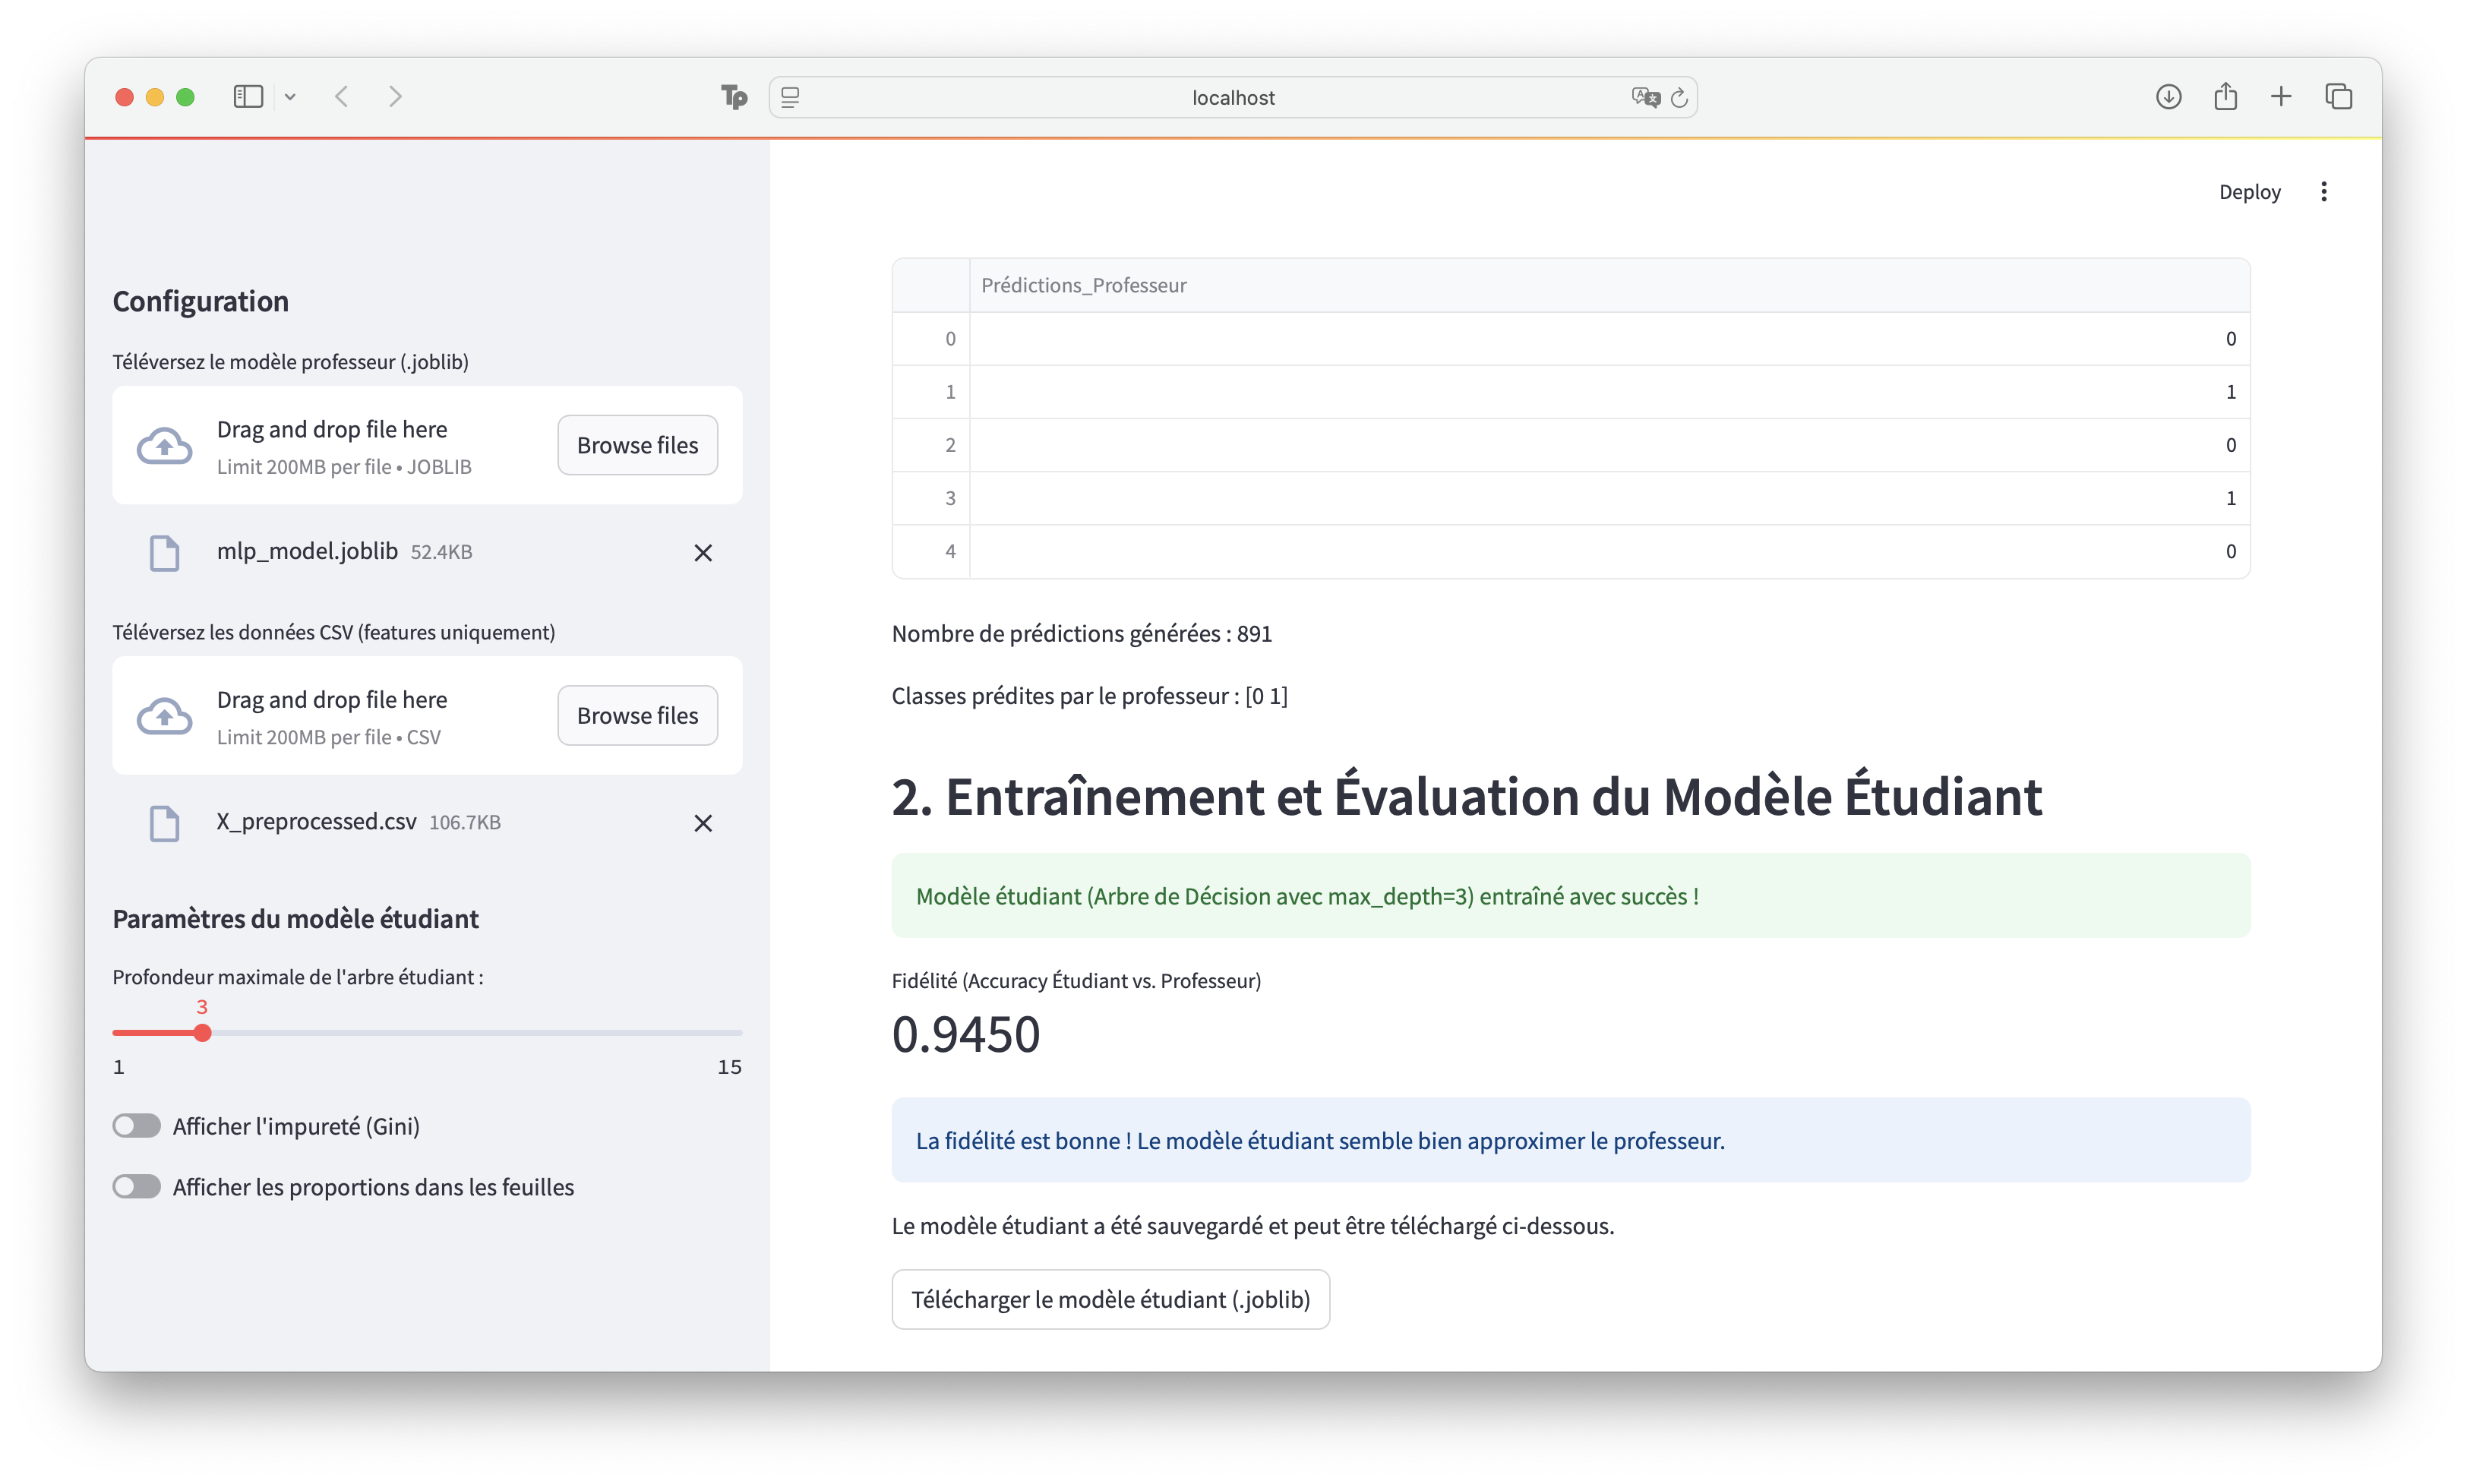
\includegraphics[width=\textwidth]{app_fidelity.png}
            \caption{Écran de résultats de l'application: affichage de la fidélité du modèle}
            \label{fig:results_view}
        \end{minipage}
        \hfill
        \begin{minipage}[b]{0.48\textwidth}
            \centering
            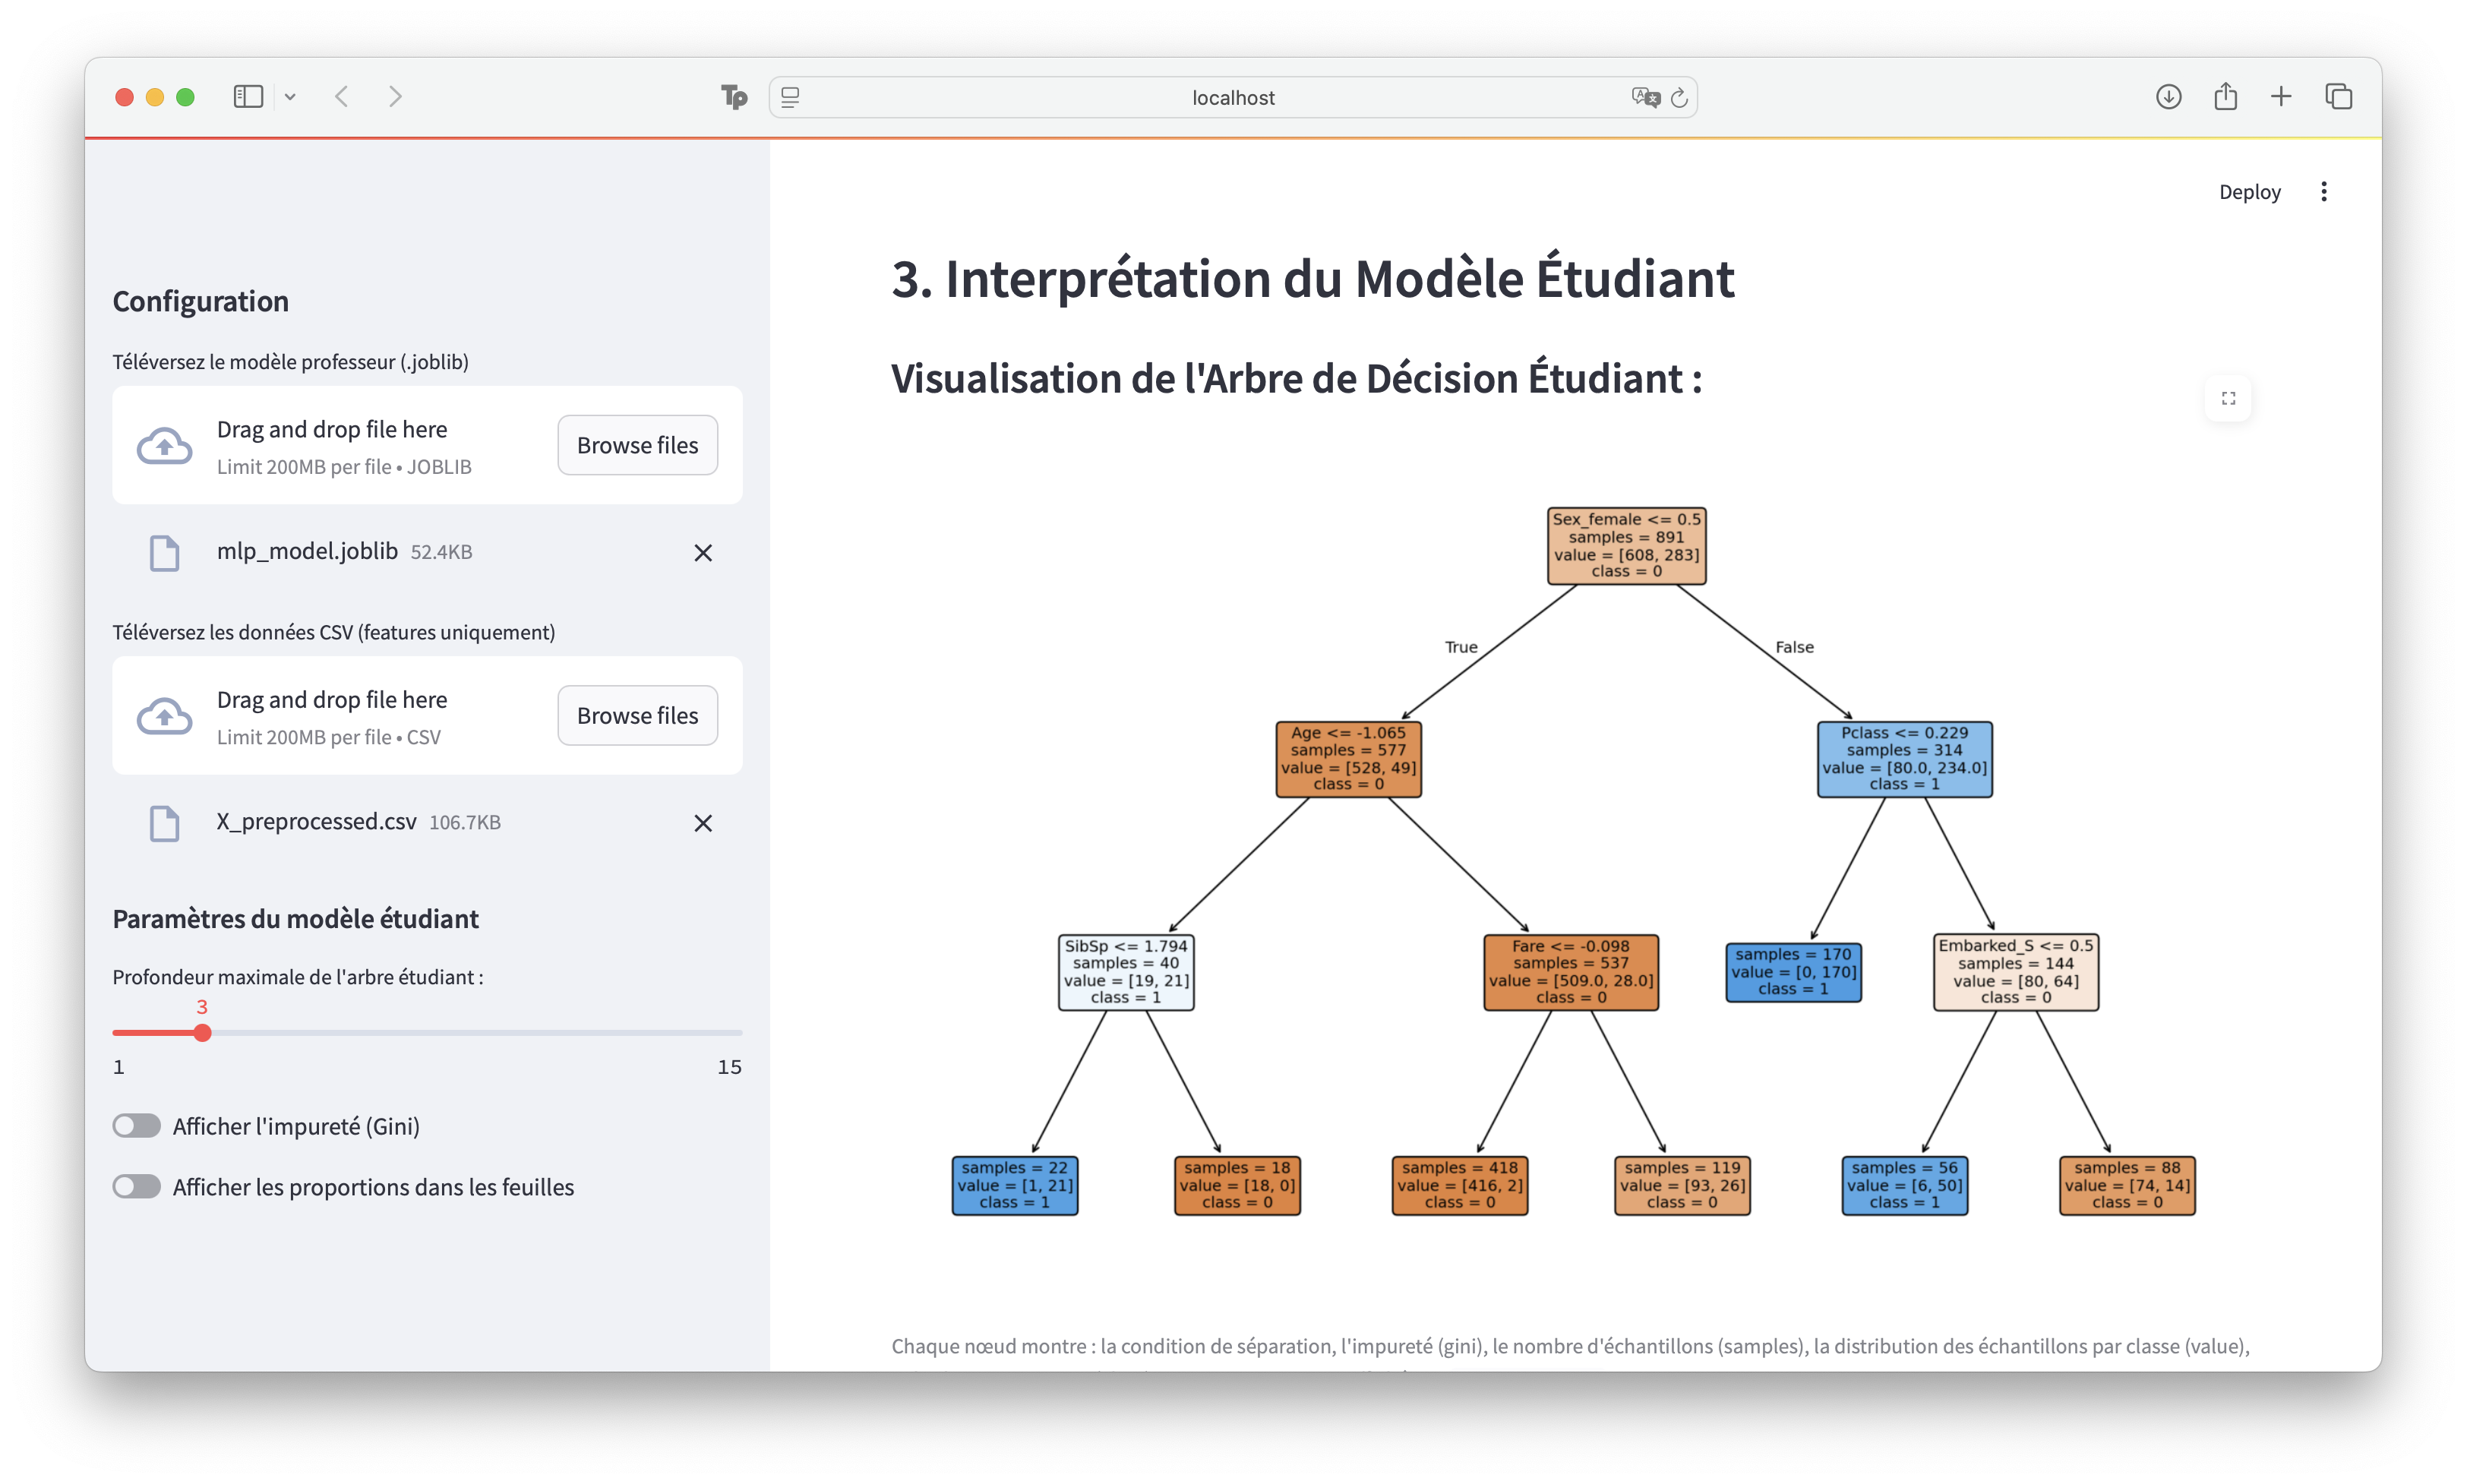
\includegraphics[width=\textwidth]{app_tree.png}
            \caption{Écran de résultats de l'application: affichage de l'arbre de décision surrogat.}
            \label{fig:input_view}
        \end{minipage}
    \end{figure}

\clearpage

\section{Résultats : Analyse de Biais sur le Dataset COMPAS}

\quad Afin de tester notre application et de pousser plus loin notre réflexion sur les biais des modèles boîte noire, nous avons mené une étude de cas sur le célèbre dataset COMPAS. L'objectif est de visualiser si un modèle entraîné sur ces données présente des disparités de traitement entre différentes ethnies, et si notre approche par modèle surrogat permet de mettre en évidence ces biais.

\subsection{Présentation Statistique du Dataset}

\quad Le jeu de données COMPAS contient des informations sur des milliers de prévenus en Floride et a été au cœur de débats sur l'équité algorithmique. Avant d'analyser les modèles, il est essentiel de comprendre la composition de ce dataset.

\begin{figure}[h!]
    \centering
    \begin{subfigure}[b]{0.48\textwidth}
        \centering
        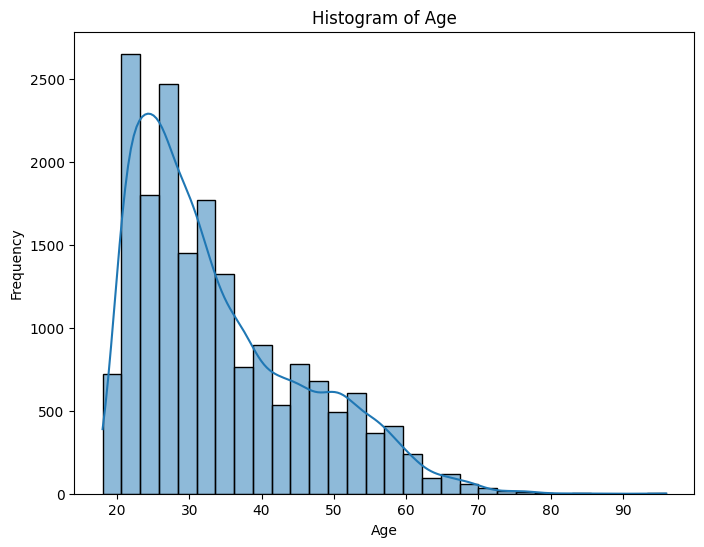
\includegraphics[width=\textwidth]{plot_age.png}
        \caption{Distribution de l'âge des prévenus.}
        \label{fig:age_distribution}
    \end{subfigure}
    \hfill
    \begin{subfigure}[b]{0.48\textwidth}
        \centering
        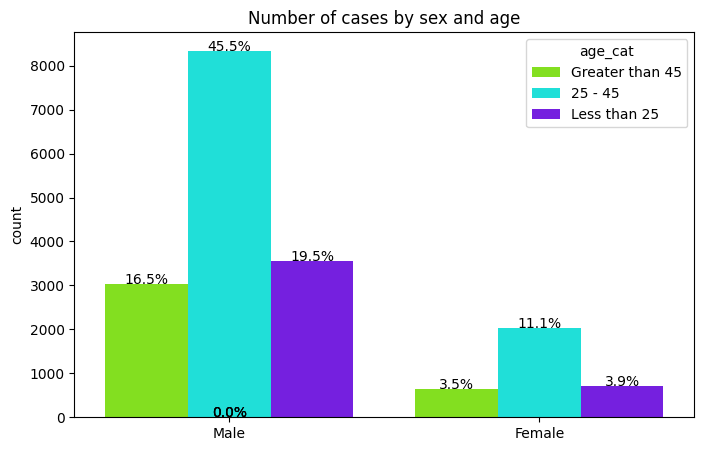
\includegraphics[width=\textwidth]{plot_sexe.png}
        \caption{Répartition des cas par sexe et catégorie d'âge.}
        \label{fig:sex_age_distribution}
    \end{subfigure}
    \caption{Statistiques démographiques du dataset COMPAS.}
\end{figure}

\quad L'histogramme de l'âge (Figure \ref{fig:age_distribution}) montre une population majoritairement jeune, avec une fréquence maximale de prévenus se situant entre 20 et 30 ans. La répartition par sexe et âge (Figure \ref{fig:sex_age_distribution}) révèle une forte prédominance masculine dans toutes les tranches d'âge, particulièrement dans la catégorie des 25-45 ans, qui représente 45,5\% des hommes contre 11,1\% des femmes.

\begin{figure}[h!]
    \centering
    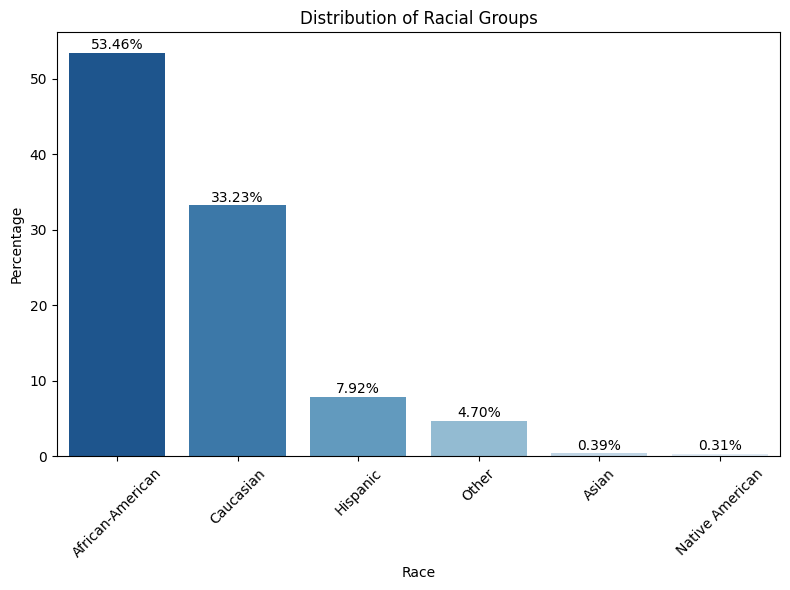
\includegraphics[width=0.57\textwidth]{plot_ethnie.png}
    \caption{Distribution des différents groupes ethniques dans le dataset.}
    \label{fig:race_distribution}
\end{figure}


\quad La Figure \ref{fig:race_distribution} illustre la répartition ethnique au sein du dataset. On observe une disparité notable : les prévenus afro-américains constituent le groupe le plus important avec 53,46\% des cas, suivis par les Caucasiens (33,23\%). Les autres groupes (Hispaniques, Asiatiques, Amérindiens et autres) sont nettement moins représentés.\\

Il est crucial de noter que ces proportions reflètent la population carcérale d'une région spécifique des États-Unis et ne sauraient être généralisées. En France, par exemple, la collecte de données ethniques est interdite par la loi, ce qui rendrait une telle analyse impossible et souligne les différences de contexte légal et social. Cette forte disproportion dans les données d'entraînement constitue un risque majeur de voir les modèles développer des biais, en associant à tort l'ethnicité au risque de récidive.

\subsection{Analyse des Biais via le Modèle Surrogat}

\quad Après avoir entraîné deux modèles de classification complexes (un Gradient Boosting Classifier et un Perceptron Multicouche) pour prédire le score de risque (`score\_text`) sur le dataset COMPAS, nous les avons soumis à notre application. L'entraînement a été volontairement naïf, avec un prétraitement minimal, en utilisant les features `age`, `c\_charge\_degree`, `race`, `sex`, `priors\_count`, et `days\_b\_screening\_arrest`. L'objectif est de voir si notre approche par modèle surrogat (un arbre de décision) peut mettre en évidence des biais dans la logique de ces boîtes noires.\\

Notre première analyse consiste à générer un arbre de décision pour approximer notre modèle boîte noire en incluant toutes les features. Avec une profondeur limitée à 4 niveaux, nous obtenons une fidélité de \textbf{86\%} par rapport au modèle professeur. Comme le montre la Figure \ref{fig:tree_lvl4}, à ce niveau d'interprétation, le modèle surrogat base principalement ses décisions sur le nombre d'antécédents judiciaires (`priors\_count`) et l'âge (`age`). Jusqu'à cette profondeur, le facteur ethnique n'apparaît pas comme un critère de décision, suggérant que le raisonnement principal du modèle n'est pas directement raciste.

\begin{figure}[h!]
    \centering
    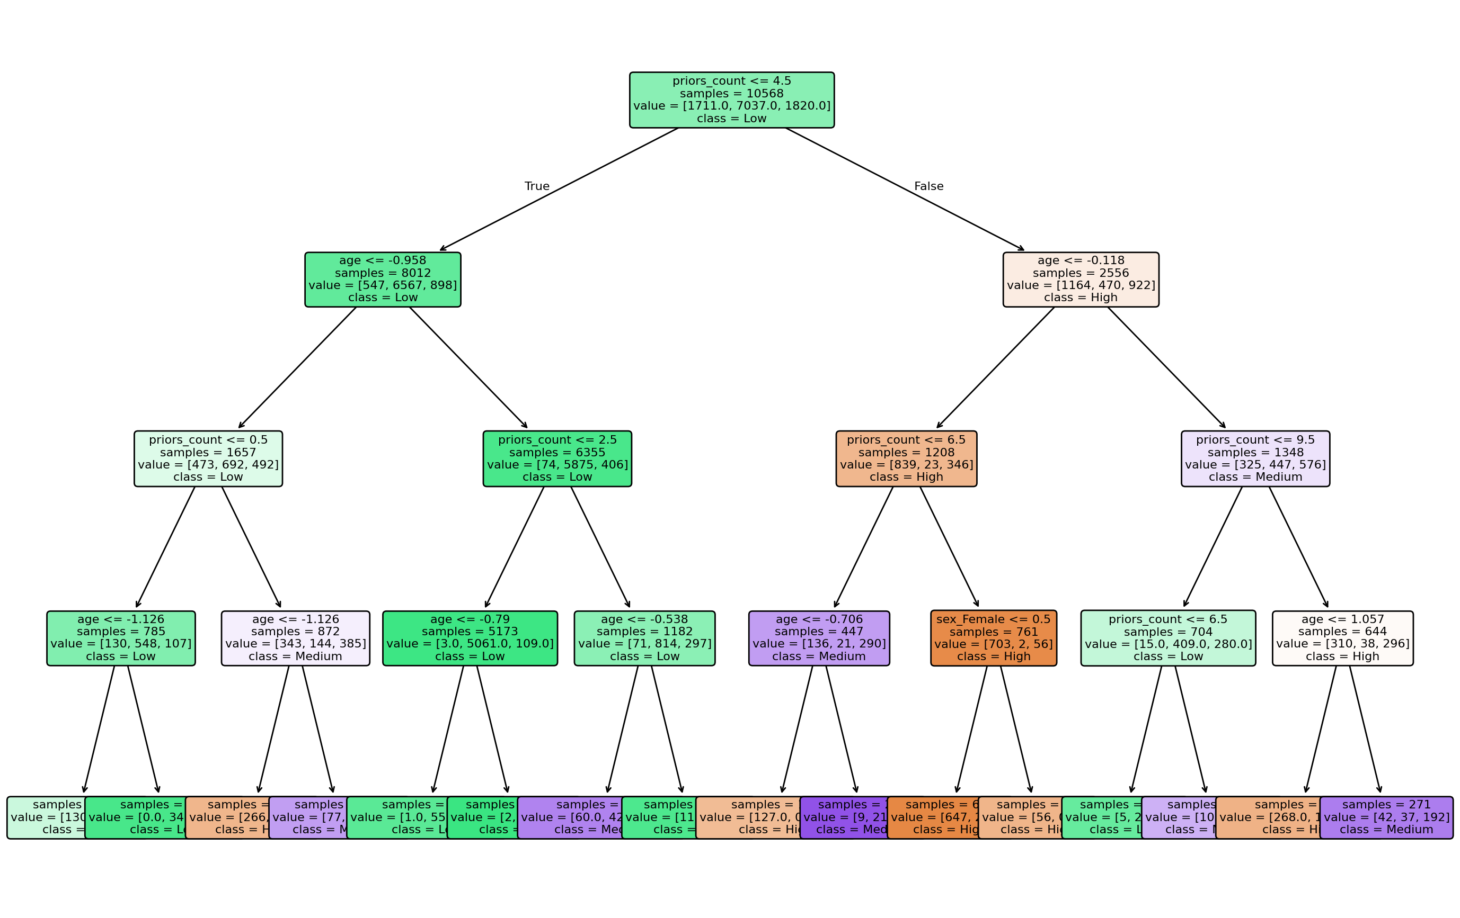
\includegraphics[width=\textwidth]{tree_with_lvl4.png}
    \caption{Arbre de décision surrogat (profondeur 4) avec une fidélité de 86\%. Les décisions principales reposent sur `priors\_count` et `age`.}
    \label{fig:tree_lvl4}
\end{figure}

\clearpage

\quad Cependant, un compromis existe entre la fidélité et la simplicité. En cherchant à augmenter la fidélité de notre approximation, nous avons augmenté la profondeur de l'arbre. En passant à une profondeur de 5, la fidélité monte à \textbf{89\%}, mais des variables démographiques commencent à apparaître dans les décisions. Ce phénomène est problématique, car il montre que pour coller plus fidèlement à la logique de la boîte noire, le modèle simple doit commencer à intégrer des facteurs potentiellement biaisés.\\

Pour pousser l'analyse plus loin, nous avons mené une seconde expérience en retirant la variable la plus prédictive, `priors\_count`, et en ré-entraînant les modèles. Le résultat, visible sur la Figure \ref{fig:tree_without_prior}, est sans équivoque. Privé de son indicateur principal, le modèle surrogat utilise maintenant les variables ethniques comme `race\_African-American` dès le deuxième niveau de l'arbre. Ce comportement est très probablement dû au fort déséquilibre du jeu de données. Pour maximiser ses chances de prédire correctement, le modèle se base sur la majorité statistique, associant ainsi l'ethnie au risque.

\begin{figure}[h!]
    \centering
    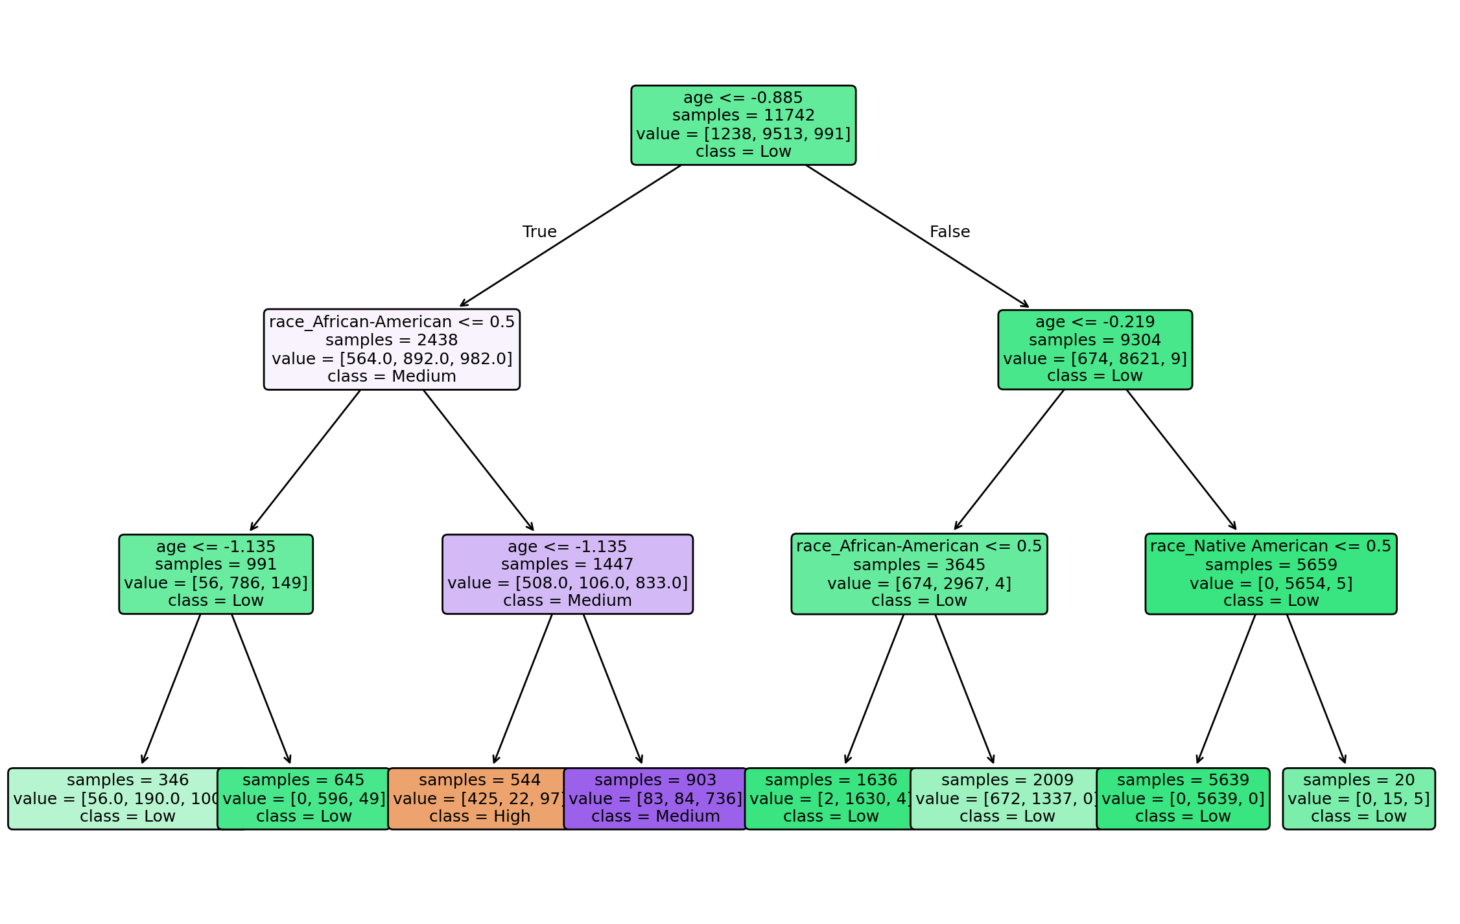
\includegraphics[width=\textwidth]{tree_withoutprior.png}
    \caption{Arbre de décision surrogat sans la feature `priors\_count`. L'ethnie (`race\_African-American`) devient un critère de décision de haut niveau.}
    \label{fig:tree_without_prior}
\end{figure}

\quad Cela prouve-t-il que le modèle est intrinsèquement raciste ? Pour le vérifier, nous avons mené un test final : ré-entraîner les modèles boîte noire originaux (Gradient Boosting et MLP) sur le jeu de données complet, mais en excluant totalement la feature `race`. De manière surprenante, les performances (accuracy, précision, rappel) de ces modèles sont restées identiques.\\

Cette dernière étape nous amène à une conclusion nuancée. Bien que le modèle puisse s'appuyer sur des biais ethniques lorsque des données plus pertinentes sont absentes ou lorsqu'on le pousse à une fidélité extrême, le facteur `race` semble être décorrélé de sa performance globale. Le modèle n'a pas besoin de l'ethnie pour effectuer ses prédictions. Le modèle n'a pas établi de lien de cause à effet, mais a détecté que cette information est statistiquement liée au résultat. Il l'utilise donc comme un substitut pratique pour prendre sa décision, surtout en l'absence de données plus directes. Notre outil permet donc non seulement de détecter un biais potentiel, mais aussi d'évaluer sa réelle importance dans la logique du modèle, offrant ainsi une vision plus juste et approfondie que la simple accusation de "biais raciste".

\clearpage

\section{Sources}

\subsection*{Concepts Généraux et Enjeux de l'Interprétabilité}

\begin{itemize}
    \item \textbf{Définition de la Boîte Noire :} Article Wikipedia fournissant la définition historique et systémique du concept de boîte noire, tel que mentionné dans notre introduction. \\
    \href{https://fr.wikipedia.org/wiki/Boîte_noire_(système)}{[Lien vers l'article]}

    \item \textbf{Le Plaidoyer pour des Modèles Interprétables :} Un article fondamental de Cynthia Rudin argumentant pourquoi, dans les domaines à forts enjeux, il est préférable d'utiliser des modèles directement interprétables plutôt que de tenter d'expliquer des boîtes noires. Cette source appuie notre mention de ses travaux. \\
    \href{https://www.nature.com/articles/s42256-019-0133-z}{[Lien vers l'article de Nature Machine Intelligence]}

    \item \textbf{Revues Générales sur l'IA Explicable (XAI) :} Une sélection d'articles de recherche qui dressent un état de l'art complet des méthodes et des défis de l'IA explicable.
    \begin{itemize}
        \item \textit{A Survey on Explainable AI (XAI): Toward Responsible AI} (MDPI, 2023) \\
        \href{https://www.mdpi.com/2078-2489/14/8/426}{[Lien vers l'article]}
        \item \textit{A survey of explainable artificial intelligence: A machine learning perspective} (Springer, 2023) \\
        \href{https://link.springer.com/article/10.1007/s12559-023-10179-8}{[Lien vers l'article]}
    \end{itemize}
\end{itemize}

\subsection*{Études de Cas sur les Domaines Critiques}

\begin{itemize}
    \item \textbf{Justice et le Scandale COMPAS :} L'enquête originelle de ProPublica, "Machine Bias", qui a révélé les biais raciaux de l'algorithme COMPAS et a été une source d'inspiration centrale pour ce projet. \\
    \href{https://www.propublica.org/article/machine-bias-risk-assessments-in-criminal-sentencing}{[Lien vers l'article de ProPublica]}

    \item \textbf{Santé et IA Médicale :} Deux articles qui illustrent les défis du déploiement de l'IA en milieu clinique, soulignant la nécessité de l'interprétabilité pour la confiance et la détection d'erreurs (comme le cas des IA pour le COVID-19).
    \begin{itemize}
        \item \textit{Deploying trustworthy AI in clinical practice requires more than just high-quality data} (Nature, 2021) \\
        \href{https://www.nature.com/articles/s42256-021-00338-7}{[Lien vers l'article]}
        \item \textit{Explainable artificial intelligence (XAI) in healthcare: A scoping review} (ScienceDirect, 2023) \\
        \href{https://www.sciencedirect.com/science/article/pii/S0933365723001732}{[Lien vers l'article]}
    \end{itemize}

    \item \textbf{Finance et Réglementation :} Sources concernant l'obligation d'expliquer les décisions algorithmiques dans le secteur financier, notamment la circulaire du CFPB américain.
    \begin{itemize}
        \item \textit{CFPB Circular on Black-Box Credit Models} (Truera, 2022) \\
        \href{https://truera.com/ai-quality-education/ai-regulation/cfpb-circular-on-black-box-credit-models-five-considerations-for-lenders}{[Lien vers l'article]}
        \item \textit{Explainable Artificial Intelligence (XAI) in the Financial Industry—A Scoping Review} (MDPI, 2023) \\
        \href{https://www.mdpi.com/2673-2688/4/2/23}{[Lien vers l'article]}
    \end{itemize}

    \item \textbf{Défense et le programme XAI de la DARPA :} La page officielle du programme XAI (Explainable Artificial Intelligence) de la DARPA, qui a financé la recherche pour rendre les systèmes militaires d'IA moins opaques. \\
    \href{https://www.darpa.mil/program/explainable-artificial-intelligence}{[Lien vers le site de la DARPA]}
\end{itemize}

\subsection*{Méthodes d'Interprétabilité (Post-Hoc et Surrogat)}

\begin{itemize}
    \item \textbf{Modèles Surrogats (Proxy Models) :} Un article de blog de RBC Borealis qui explique clairement le concept de modèle surrogat global, au cœur de notre application. \\
    \href{https://rbcborealis.com/research-blogs/explainability-ii-global-explanations-proxy-models-and-interpretable-models/}{[Lien vers l'article de RBC Borealis]}

    \item \textbf{Méthodes Post-Hoc (LIME et SHAP) :} Les publications scientifiques originales présentant les méthodes LIME et SHAP, les deux approches post-hoc les plus influentes citées dans notre état de l'art.
    \begin{itemize}
        \item \textit{LIME: "Why Should I Trust You?": Explaining the Predictions of Any Classifier} (Ribeiro, Singh, Guestrin, 2016) \\
        \href{https://arxiv.org/abs/1602.04938}{[Lien vers l'article sur arXiv]}
        \item \textit{SHAP: A Unified Approach to Interpreting Model Predictions} (Lundberg, Lee, 2017) \\
        \href{https://arxiv.org/abs/1705.07874}{[Lien vers l'article sur arXiv]}
    \end{itemize}

    \item \textbf{Approches Techniques des Modèles Surrogats :} Un article de recherche plus technique sur une méthode post-hoc basée sur un modèle surrogat et la théorie des jeux. \\
    \href{https://www.sciencedirect.com/science/article/abs/pii/S0925231224007409}{[Lien vers l'article de ScienceDirect]}
\end{itemize}

\end{document}
